\documentclass[a4paper,12pt]{article}

%------------------------------------------------------------------------------------------%
% Déclaration des packages
%------------------------------------------------------------------------------------------%

\usepackage[french]{babel}
\frenchbsetup{StandardLists=true}
\usepackage{enumitem}
\usepackage[T1]{fontenc}
\usepackage{geometry} % pour gérer les dimensions des marges
\usepackage{eso-pic} % pour dessiner la marge
\usepackage{lipsum} % pour générer du contenu texte
\usepackage[cyr]{aeguill} % Police vectorielle TrueType, guillemets fran¸cais
\usepackage{epsfig} % pour g´erer les images
\usepackage{amsmath, amsthm} % tr`es bon mode math´ematique
\usepackage{amsfonts,amssymb}% permet la definition des ensembles
\usepackage{float} % pour le placement des figure
\usepackage{url} 
\usepackage[utf8]{inputenc}
\usepackage{amssymb}
\usepackage{graphicx}
\usepackage{ulem}
\usepackage{array}	
\usepackage{listings}
\usepackage{siunitx}
\usepackage{fancybox}
\usepackage{wrapfig}
\usepackage{caption}
 \usepackage{hyperref}
\usepackage{listings}
\usepackage{xcolor}
\usepackage{booktabs}
\usepackage{fancyhdr}
\usepackage{tabularx}
\usepackage[style=authoryear,backend=biber]{biblatex}
\addbibresource{biblio.bib} 

\lstdefinelanguage{Dockerfile}{
  keywords={FROM, RUN, CMD, LABEL, MAINTAINER, EXPOSE, ENV, ADD, COPY, ENTRYPOINT, VOLUME, USER, WORKDIR, ARG, ONBUILD, STOPSIGNAL, HEALTHCHECK, SHELL},
  keywordstyle=\color{blue}\bfseries,
  identifierstyle=\color{black},
  sensitive=false,
  comment=[l]{\#},
  commentstyle=\color{gray}\ttfamily,
  stringstyle=\color{green},
  morestring=[b]",
  morestring=[b]',
}

\lstdefinelanguage{Python}{
  keywords={True, False, None, await, break, class, def, if, else, elif, for, while, continue, return, and, or, not, in, is, try, except, finally, raise, assert},
  keywordstyle=\color{blue}\bfseries,
  ndkeywords={import, from, as, with, print, yield},
  ndkeywordstyle=\color{darkgray}\bfseries,
  identifierstyle=\color{black},
  comment=[l]{\#},
  commentstyle=\color{green}\ttfamily,
  stringstyle=\color{green},
  morestring=[b]',
  morestring=[b]",
  sensitive=true,
}


\pagestyle{fancy}
\fancyhf{} % Efface les configurations précédentes
\fancyhead[L]{AI referent apprenticeship} % Titre du rapport à gauche
\fancyhead[C]{SAPLABS} % Numéro de page au centre
\fancyhead[R]{HADDOU Amine} % Nom de l'auteur à droite
\fancyfoot[R]{\thepage} % Numéro de page au centre
\fancyfoot[L]{Master 1 informatique\\parcours Intelligence Artificielle} % Numéro de page au centre

\geometry{top=25mm, bottom=25mm, left=20mm, right=1cm}
\setlength\headheight{10mm}
\DeclareUnicodeCharacter{2212}{-}
\renewcommand{\thefootnote}{\fnsymbol{footnote}}
\renewcommand{\thefootnote}{\fnsymbol{footnote}}
\newcommand{\chatgptprompt}[1]{
    \vspace{10pt}
    \noindent\textbf{ChatGPT Prompt:}\\
    \fbox{
        \parbox{\textwidth}{
            \texttt{#1}
        }
    }
    \vspace{10pt}
}



\geometry{a4paper, margin=1in}

\title{\huge\bf  Rapport d'alternance}
\author{HADDOU Amine} 
\begin{document}

\begin{titlepage}
    \begin{center}
        
\includegraphics[width=0.5\textwidth]{./images/logo_master.png}\\
        
\includegraphics[width=0.3\textwidth]{./images/DS4HlogocouleurFR.png} \hfill
        
\includegraphics[width=0.10\textwidth]{./images/tampon-3IA.png} \hfill
        \textbf{
\includegraphics[width=0.3\textwidth]{./images/cfa.png}} \\
        
        \vspace{1.5cm}
        
        \textbf{\LARGE Université C\^ote d'Azur}
        
        \vspace{0.5cm}
        
        \textbf{\Large MASTER INFORMATIQUE\\ Parcours INTELLIGENCE ARTIFICIELLE}
        
        \vspace{1.5cm}
        
        \rule{\linewidth}{0.5mm} \\[0.4cm]
        {\LARGE \bfseries Algorithme de recommendation - Projet TATIA\\[0.5cm] }
        \rule{\linewidth}{0.5mm} \\[1.5cm]
        
        \textbf{Authors:}\\ BOULLI Marouan \& HADDOU Amine \\
        
        \vspace{0.5cm}
        
        \textbf{Mentor:} \\
        CABRIO Elena\\
       
        
    \end{center}
\end{titlepage}

\newpage
\maketitle
\tableofcontents

\newpage

\section{Recommandation d'articles}

Comme sujet de projet, nous avons choisi d'implémenter un algorithme de recommandation d'articles en fonction du dernier article lu par l'utilisateur. Le fonctionnement de cet algorithme se décompose en deux étapes principales : classifier l'article et fournir un classement d'articles similaires au dernier lu.\\

Concernant la classification, nous travaillerons avec 5 catégories d'articles différentes. Ce choix a été imposé par le jeu de données trouvé, mais ces catégories englobent un ensemble d'articles riche et diversifié. Les catégories sont \textit{business}, \textit{entertainment}, \textit{politics}, \textit{sport}, et \textit{tech}.\\

Une fois l'article classifié, l'algorithme proposera un classement des 3 articles les plus similaires dans notre jeu de données. Notre classement sera basé sur un calcul de similarité de l'article lu comparé aux autres articles de la même catégorie.\\

On pourrait alors se demander quelle est l'utilité de classifier l'article. Dans un contexte d'une large base de données, il est important de prendre en compte le coût et la consommation de calcul de similarité sur un grand ensemble d'articles différents. De plus, nous souhaitons que les articles recommandés appartiennent à la même catégorie que le dernier article lu par l'utilisateur. Nous implémenterons l'algorithme dans cette logique.\\

Enfin, nous devrons valider notre algorithme pour en juger l'efficacité. Pour ce faire, nous baserons la validation sur deux métriques : l'\textit{accuracy} et le ratio de mots clés similaires entre les articles.\\

\section{Jeu de données}

Comme base de données pour ce projet, nous avons choisi le jeu de données d'articles de la BBC disponible sur \href{https://www.kaggle.com/c/learn-ai-bbc}{Kaggle}.\\

Le jeu de données est décomposé en deux ensembles : un ensemble de \textit{training} contenant 1490 articles, et un second de \textit{testing} contenant 735. La différence entre les deux ensembles réside dans la classification des articles. Les articles du premier ensemble sont labellisés alors que ceux du second ne le sont pas. Pour cette raison, nous nous limiterons à travailler avec le premier ensemble pour le moment. Nous n'utiliserons le second que lors de la validation pour tester les performances de l'algorithme final.\\

Il est ensuite important de vérifier que le jeu de données n'est pas biaisé en sur-représentant ou sous-représentant une catégorie. Notre jeu de données est bien équilibré, avec des catégories représentant entre $17.5\%$ et $23.3\%$ de l'ensemble des données, comme le montre la Figure \autoref{fig:classBalance}.

\begin{figure}[h]
  \centering
  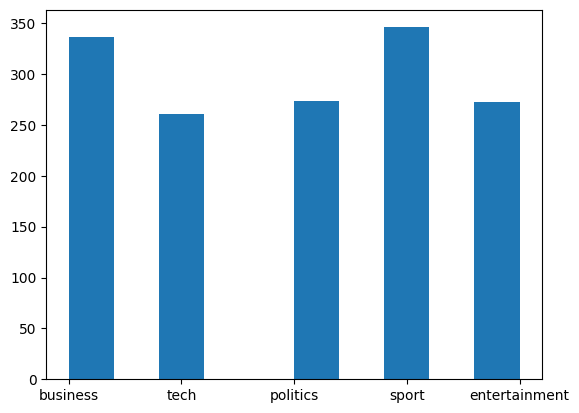
\includegraphics{./images/class_balanced.png} % Spécifiez le chemin de votre image
  \caption{Proportion des catégories d'articles}
  \label{fig:classBalance}
\end{figure}

\subsection{Prétraitement}

Avant d'entamer l'implémentation de l'algorithme, il est essentiel de débuter par le prétraitement de notre jeu de données. Cette phase est cruciale, car elle conditionne la qualité de nos données et, par conséquent, celle de notre algorithme.\\

Il convient de souligner que notre jeu de données est prêt à être traité. Les modèles de machine learning présentent des performances médiocres avec des données textuelles brutes. L'objectif principal est de surmonter cette contrainte en apportant des modifications subtiles à notre base de données.\\

Nous commencerons par éliminer la ponctuation des articles, car elle ne contribue pas à la valeur sémantique de la classification. Ensuite, nous supprimerons les mots dépourvus de sens sémantique, tels que les articles et les prépositions. Voici un exemple des modifications apportées :

\textit{``WorldCom ex-boss launches defense. Lawyers defending former WorldCom chief Bernie Ebbers against a battery of fraud charges have called a company whistleblower as their first witness.''}

\textit{``WorldCom ex-boss launches defense. Lawyers defending former WorldCom chief Bernie Ebbers battery fraud charges called company whistleblower first witness.''}\\

Enfin, nous réaliserons une lemmatisation pour nous concentrer uniquement sur le sens global de l'article. Ce procédé nous permettra de mettre en évidence les mots clés, de normaliser le texte et d'améliorer la précision sémantique des modèles de machine learning. Nous utiliserons le lemmatizer \textit{WordNetLemmatizer}, entraîné sur la base de données \textit{WordNet}, pour lemmatiser notre jeu de données. Appliqué sur l'exemple précédent, nous obtenons :

\textit{``WorldCom ex-boss launch defense lawyer defend former WorldCom chief Bernie Ebbers battery fraud charge call company whistleblower first witness.''}

Enfin, nous vectoriserons les articles transformés pour obtenir un jeu de données adapté au machine learning. Cette étape sera réalisée dans un pipeline présenté dans la section suivante.

\section{Entraînement des modèles}

Afin de classifier les articles, nous testerons différents modèles de classification. Mais avant cela, il nous reste une dernière étape : diviser notre jeu de données en deux parties. La première sera utilisée pour l'entraînement et la seconde pour les tests. Il est recommandé, pour un jeu de données de notre envergure, de conserver $77\%$ du dataset pour l'entraînement et le reste pour les tests, ce que nous appliquerons ici.

\subsection{Support Vector Machine Classifier}

Le premier modèle choisi est le Support Vector Machine Classifier. Ce modèle est généralement utilisé sur des datasets de taille moyenne (quelques milliers), mais il peut également être très performant sur des jeux de données de qualité plus restreints.


\subsubsection{Pipeline}

Pour l'entraînement, nous créons deux pipelines permettant d'automatiser une série de tâches. Chaque pipeline se charge de :
\begin{itemize}
    \item Vectoriser les articles grâce à la classe \texttt{CountVectorizer} fournie par \textit{Scikit-learn}.
    \item \textit{TfidfTransformer} : calcule le poids des mots dans chaque phrase en fonction de leur fréquence dans le corpus.
    \item Entraîner le modèle SVC sur le jeu de données modifié.
\end{itemize}

La deuxième pipeline est la suivante :
\begin{itemize}
    \item Vectoriser les articles grâce à la classe \texttt{CountVectorizer} fournie par \textit{Scikit-learn}.
    \item \textit{Doc2Vec} : une méthode donnant un poids aux mots en se basant sur des réseaux de neurones.
    \item Entraîner le modèle SVC sur le jeu de données modifié.
\end{itemize}

\subsubsection{Validation}

Pour valider un modèle, nous nous baserons sur les métriques proposées par Scikit-learn : l'accuracy et la précision principalement. En utilisant les deux pipelines, on obtient les mêmes résultats sauf pour l'accuracy. On gagne 1\% de plus en score en utilisant \textit{Doc2Vec} : 98\% contre 97\%.

\subsection{K-Neighbors Classifier}

Le second modèle choisi est le K-Neighbors Classifier. Ce modèle peut performer correctement sur notre dataset, mais il est généralement plus lent que le précédent.

\subsubsection{Pipeline}

Pour l'entraînement, nous reprenons les deux pipelines présentées précédemment.

\subsubsection{Validation}

En utilisant les deux pipelines, on obtient de moins bons résultats en utilisant le \textit{TF-IDF} (95\% d'accuracy). Alors qu'avec \textit{Doc2Vec}, on obtient des résultats similaires à ceux du SVM entraîné avec une pipeline \textit{TF-IDF}.

\section{Recommandation d'articles}

Dans cette section, nous nous intéressons à la seconde tâche de notre algorithme : la recommandation d'articles similaires.

\subsection{Cosine Similarity}

Pour calculer la similarité entre deux articles, nous avons utilisé la métrique \textit{cosine similarity} fournie par la librairie \textit{Scikit-Learn} en Python. Nous avons calculé cette métrique entre l'article de l'utilisateur et tous les articles filtrés à l'étape précédente. Enfin, nous avons sélectionné seulement les trois articles ayant la plus grande valeur.\\

Notre algorithme recommandera alors ces trois articles qu'il considérera comme les plus proches de l'original.

\subsection{Évaluation}

Après avoir implémenté cette méthode, il nous fallait l'évaluer. Quelle est la cohérence des recommandations ? Pour cela, nous avons utilisé deux méthodes différentes. Un de nos objectifs secondaires était de trouver une manière d'automatiser cette évaluation, car habituellement elle est manuelle.

\subsubsection{Évaluation par extraction de mots-clés}

La première méthode que nous avons utilisée est l'extraction de mots-clés. Nous avons extrait les mots-clés de chaque document en utilisant une fonction proposée par la librairie \textit{yake}.\\

Nous avons ensuite calculé la similarité entre les articles en nous basant sur le nombre de mots-clés en commun.\\

Pour calculer l'accuracy de notre méthode, nous sommes partis du principe que si \textbf{un} des 3 articles recommandés figurait parmi les articles similaires (selon la méthode d'extraction de mots-clés), alors la recommandation était bonne.\\

Nous avons alors obtenu une accuracy de 34\%.

\subsubsection{Évaluation par LLM}

Cette méthode n'étant pas satisfaisante, nous avons décidé de tester une autre manière d'évaluer nos résultats en utilisant de grands modèles de langage. Dans le cadre de cette évaluation, nous avons utilisé OPENAI-GPT4, Claude AI, GEMINI et Mistral AI.\\

Nous leur avons fourni un article utilisateur et 10 autres articles aléatoires de la même catégorie. Nous leur avons ensuite demandé de retourner les 3 articles les plus similaires selon eux.\\

Tous les LLM ont retourné quasiment les 2 premiers articles et ont chacun proposé un article différent pour la 3ème position. Malheureusement, seul le 3ème article proposé par Gemini a été recommandé par notre algorithme.

\subsubsection{Évaluation manuelle}

Toutefois, ces méthodes d'évaluation ne sont pas parfaites et les résultats ne sont pas concluants. En effet, l'extraction de mots-clés pour évaluer la similarité entre deux articles est une méthode moins efficace que la \textit{cosine similarity}. De même, le classement des articles de recommandations par les LLM n'a pas de grande valeur, car on ne sait pas comment cette évaluation est effectuée.\\

Le meilleur moyen d'évaluer l'algorithme est de le tester manuellement avec des utilisateurs réels. Les résultats obtenus seront alors plus concluants et cohérents pour évaluer notre modèle.


\section{Conclusion}














































\end{document}